\section{Layout construction}\label{sec:layout-construction}

This section describes the process of how to transform or decode an individual.
This transformation aims to create a solution to the painting placement problem,
which is a set of placement points for the paintings.
There are multiple steps to this process which are described in the following subsections
– decoding random keys and orientation probabilities in~\ref{subsec:individual-decoding},
slicing layout construction in~\ref{subsec:slicing-tree-construction},
and greedy placement heuristic in~\ref{subsec:placement-heuristics}.

\subsection{Individual decoding}\label{subsec:individual-decoding}
First, we must decode an individual to the representation from which a slicing layout can be constructed.
Decoded individual is composed of (1) painting sequence, (2) slicing order, and (3) orientations.
An example of individual decoding is in figure~\ref{fig:individual-decoding}.

Let us use the notation for painting sequence as $PS$, slicing order as $SO$, orientations $OR$.
$PS$ contains painting identifiers, $SO$ contains information used to construct slicing layout,
and $OR$ contains type of the cuts in the slicing layout – $H$ for horizontal, $V$ for vertical
and $*$ for wildcard, that can take up any value $H$ or $V$.

\subsubsection*{Random keys decoding}
Decoding both $PS_{rk}$ and $SO_{rk}$ is the same as the RKGA in~\cite{beanGeneticAlgorithmsRandom1994}.
Graphical illustration is in figure~\ref{fig:individual-decoding} marked as~\textit{random key decoder}.
Decoding random keys can be explained in the following steps on a sequence of four numbers $S = 0.3, 0.2, 0.4, 0.1$\,.

\begin{enumerate}
    \item Create $S'$ by adding lower index to each element from $S$ which marks its ordinal position starting from one.
    $S' = 0.3_1, 0.2_2, 0.4_3, 0.1_4$\,.
    \item Sort $S'$ in descending order. $S' = 0.1_4, 0.2_2,  0.3_1, 0.4_3$\,.
    \item Take lower indexes of $S'$.
    It is the result – $4, 2, 1, 3$.
\end{enumerate}


\subsubsection*{Orientation probabilities decoding}

Last part of the individual, matrix $OR_{prob} \in \real^{N-1, 3}$, decodes to the sequence of symbols from $\Sigma = \{H, V, *\} $.
The graphical illustration is in figure~\ref{fig:individual-decoding} marked as~\textit{orientation decoder}.

Decoding $OR_{prob}$ translates each row to one symbol from $\Sigma$, producing a symbol sequence.
Thus, decoding orientation probabilities can be explained for one row, say $R = 0.7, 0.2, 0.1$
in the following steps.


\begin{enumerate}
    \item Create $R'$ by adding lower index $H$ to the first, $V$ to the second, and $*$ to the last $R$'s elements.
    $R' = 0.7_H, 0.2_V, 0.1_*$
    \item Select element from $R'$ with the maximum value. $\max R' = 0.7_H$.
    \item Take lower index of $\max R'$.
    It is the result – $H$.
\end{enumerate}

There is one exception to the steps described above.
It is the limit on the maximum number of $*$ symbols produced by orientation probabilities decoding.
Let us call this limit $k$.
If the limit is not applicable, i.e., $k \geq N-1$, there is no change to steps 1--3 described above.
However, if applicable, only the first $k$ symbols $*$ with the highest probability are considered.
It is achieved by setting probability to $0$ (only for the duration of the decoding) to the bottom $N-1-k$ symbols $*$ with the lowest probability.
Then the same 1--3 steps are applied as described above.

One example where the limit applies is for the $k=1$ and $OR_{prob}$ that has two rows, $R_1 = 0.2, 0.3, 0.5$ and $R_2 = 0.1, 0.2, 0.7$.
Without exception, the result is $*, *$.
However, considering the exception on the maximum limit $k=1$, the result is $V, *$.
Reason is that in $R_2$, symbol $*$ has probability $0.7$,
which is higher than probability of $*$ in $R_1$, which is $0.5$.



\begin{figure}[htp]
    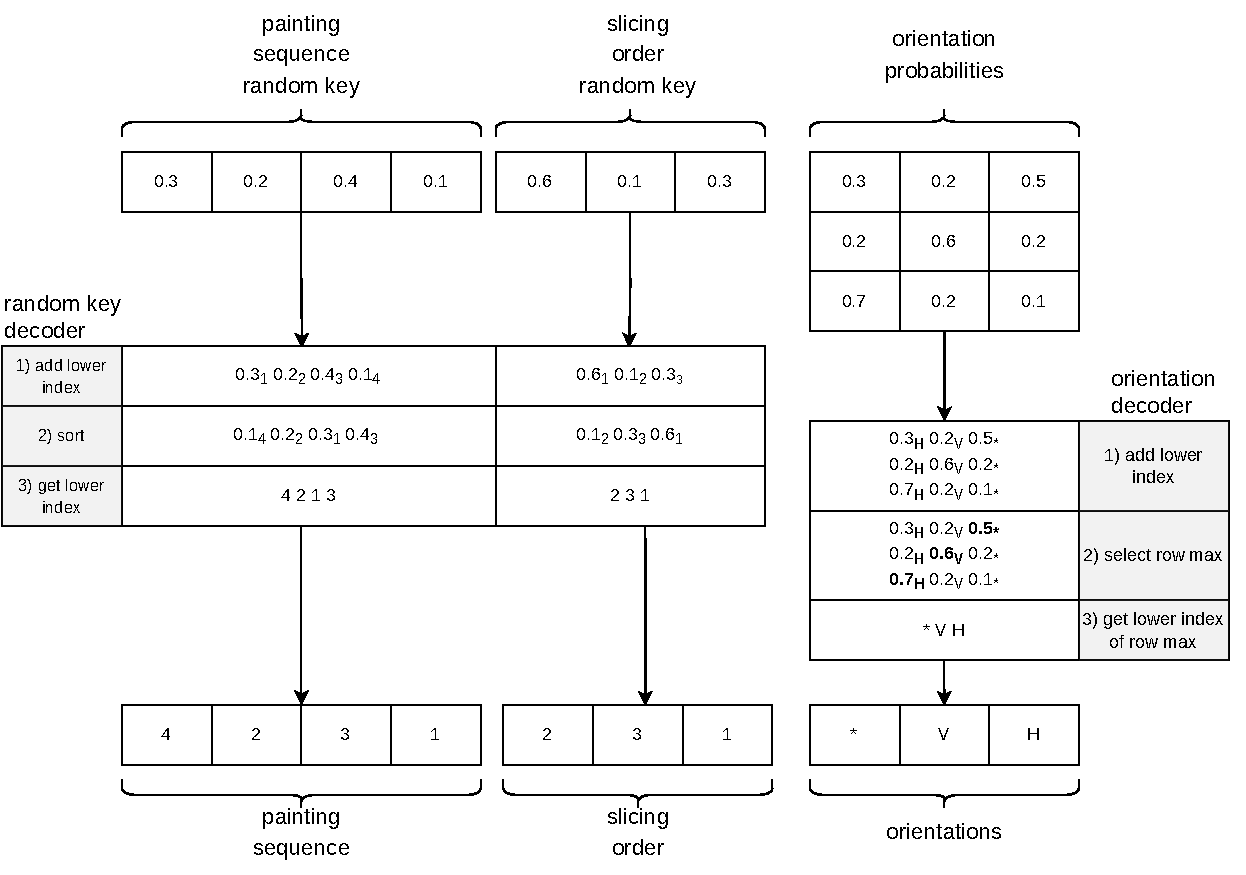
\includegraphics[width=1.1\textwidth, left]{individual_decoding}
    \caption{
        Individual decoding example. Both the painting sequence random key and slicing order random key
        are decoded using the same procedure. The decoded individual can be used to construct a slicing tree.
    }
    \label{fig:individual-decoding}
\end{figure}

\subsection{Slicing layout construction}\label{subsec:slicing-tree-construction}

\afterpage{%
    \clearpage% Flush earlier floats (otherwise order might not be correct)
    \begin{landscape}% Landscape page
        \begin{figure}[]
            \centering
            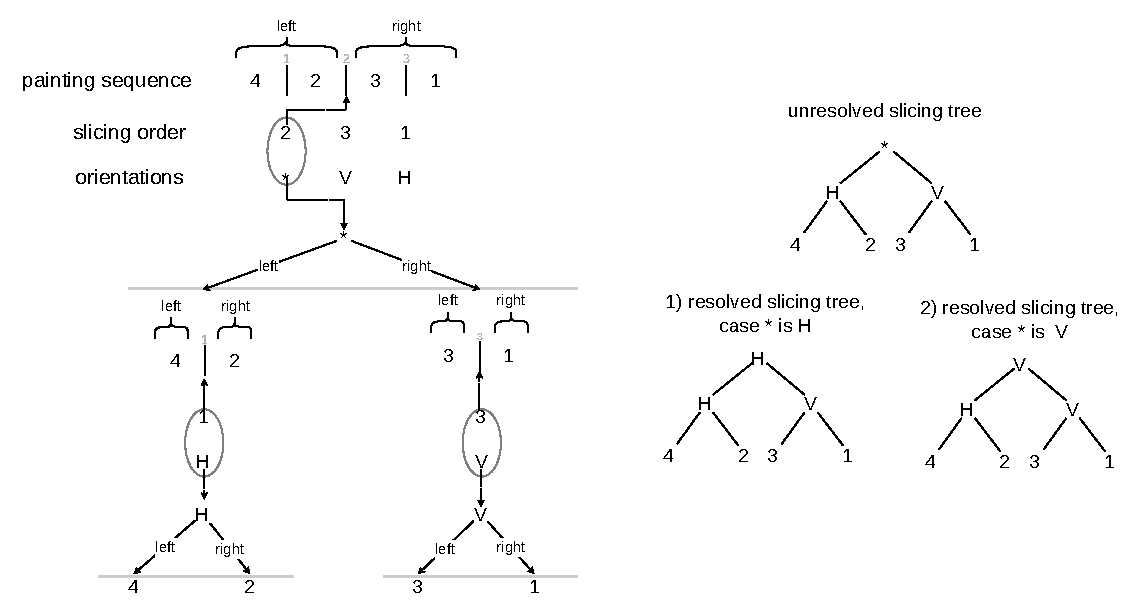
\includegraphics[width=1.5\textwidth]{slicing_tree_construction}
            \caption{
                Slicing tree and slicing layout construction from a decoded individual.
                On the left is the process of constructing an unresolved slicing tree.
                On the right are an unresolved slicing tree, and two resolved slicing trees that it represents together with corresponding slicing layouts.}
            \label{fig:slicing-tree-construction}
        \end{figure}
    \end{landscape}
    \clearpage% Flush page
}

\subsection{Placement heuristics}\label{subsec:placement-heuristics}